% Class option set by build_profiles.sh; the content does not depend on it:
%   conference : formato de congreso (HRFEST)
%   journal    : formato de revista IEEE
\ifdefined\PAPERCLASSOPT\else\def\PAPERCLASSOPT{conference}\fi
\documentclass[\PAPERCLASSOPT]{IEEEtran}
\IEEEoverridecommandlockouts

\usepackage{cite}
\usepackage{amsmath,amssymb}
\usepackage{graphicx}
\usepackage{booktabs}
\usepackage{url}
\newcommand{\PaperTitle}{Evaluating UAV Coverage Plans Beyond Path Length Using Embedded-Deployable Nonlinear Model Predictive Control}
\newcommand{\PaperAuthors}{Jose Luis Segundo Manayay, Javier Yanpier Garay Yovera, Francisco Jes\'us Rodr\'iguez Huiman, Luis Angel Vilcamiche Fernandez}
\newcommand{\PaperAuthorsPDF}{Jose Luis Segundo Manayay, Javier Yanpier Garay Yovera, Francisco Jes\string\372s Rodr\string\355guez Huiman, Luis Angel Vilcamiche Fernandez}
\usepackage{microtype}
\usepackage[T1]{fontenc}
\usepackage[utf8]{inputenc}
\usepackage{xcolor}
% PDF profiles from one source.
%   interactive: blue mailto/DOI/URL links and a clickable ORCID logo.
%   ieee (default): no link annotations and no bookmarks, for IEEE PDF eXpress;
%   metadata written with \pdfinfo; ORCID logo kept as plain vector art.
% Select with \def\PDFPROFILE{interactive} before % Class option set by build_profiles.sh; the content does not depend on it:
%   conference : formato de congreso (HRFEST)
%   journal    : formato de revista IEEE
\ifdefined\PAPERCLASSOPT\else\def\PAPERCLASSOPT{conference}\fi
\documentclass[\PAPERCLASSOPT]{IEEEtran}
\IEEEoverridecommandlockouts

\usepackage{cite}
\usepackage{amsmath,amssymb}
\usepackage{graphicx}
\usepackage{booktabs}
\usepackage{url}
\newcommand{\PaperTitle}{Evaluating UAV Coverage Plans Beyond Path Length Using Embedded-Deployable Nonlinear Model Predictive Control}
\newcommand{\PaperAuthors}{Jose Luis Segundo Manayay, Javier Yanpier Garay Yovera, Francisco Jes\'us Rodr\'iguez Huiman, Luis Angel Vilcamiche Fernandez}
\newcommand{\PaperAuthorsPDF}{Jose Luis Segundo Manayay, Javier Yanpier Garay Yovera, Francisco Jes\string\372s Rodr\string\355guez Huiman, Luis Angel Vilcamiche Fernandez}
\usepackage{microtype}
\usepackage[T1]{fontenc}
\usepackage[utf8]{inputenc}
\usepackage{xcolor}
% PDF profiles from one source.
%   interactive: blue mailto/DOI/URL links and a clickable ORCID logo.
%   ieee (default): no link annotations and no bookmarks, for IEEE PDF eXpress;
%   metadata written with \pdfinfo; ORCID logo kept as plain vector art.
% Select with \def\PDFPROFILE{interactive} before \input{main.tex}.
% Requires \PaperTitle, \PaperAuthors (UTF-8, hyperref) and \PaperAuthorsPDF
% (PDFDocEncoding octal escapes, \pdfinfo) to be defined first.
\ifdefined\PDFPROFILE\else\def\PDFPROFILE{ieee}\fi
\def\profileinteractive{interactive}
\usepackage{tikz}
\usetikzlibrary{svg.path}
\definecolor{orcidlogocol}{HTML}{A6CE39}
% ORCID iD logo, same artwork as the orcidlink package (vector, no Type 3).
\newlength{\orcidxheight}
\newcommand{\orcidlogo}{\setlength{\orcidxheight}{\fontcharht\font`X}%
  \mbox{\begin{tikzpicture}[yscale=-0.00390625*\orcidxheight,
      xscale=0.00390625*\orcidxheight,transform shape]
    \fill[orcidlogocol] svg{M256,128c0,70.7-57.3,128-128,128C57.3,256,0,198.7,0,128C0,57.3,57.3,0,128,0C198.7,0,256,57.3,256,128z};
    \fill[white] svg{M86.3,186.2H70.9V79.1h15.4v48.4V186.2z}
      svg{M108.9,79.1h41.6c39.6,0,57,28.3,57,53.6c0,27.5-21.5,53.6-56.8,53.6h-41.8V79.1z M124.3,172.4h24.5c34.9,0,42.9-26.5,42.9-39.7c0-21.5-13.7-39.7-43.7-39.7h-23.7V172.4z}
      svg{M88.7,56.8c0,5.5-4.5,10.1-10.1,10.1c-5.6,0-10.1-4.6-10.1-10.1c0-5.6,4.5-10.1,10.1-10.1C84.2,46.7,88.7,51.3,88.7,56.8z};
  \end{tikzpicture}}}
\ifx\PDFPROFILE\profileinteractive
  \usepackage[colorlinks=true,linkcolor=black,citecolor=black,urlcolor=blue,
              bookmarks=false]{hyperref}
  \hypersetup{pdftitle={\PaperTitle},pdfauthor={\PaperAuthors}}
  \newcommand{\orcid}[1]{\href{https://orcid.org/#1}{\orcidlogo}}
  \newcommand{\authoremail}[1]{\href{mailto:#1}{#1}}
  \newcommand{\doititle}[2]{\href{https://doi.org/#1}{#2}}
  \newcommand{\urltitle}[2]{\href{#1}{#2}}
\else
  \pdfinfo{/Title (\PaperTitle) /Author (\PaperAuthorsPDF)}
  \newcommand{\orcid}[1]{\orcidlogo}
  \newcommand{\authoremail}[1]{#1}
  \newcommand{\doititle}[2]{#2}
  \newcommand{\urltitle}[2]{#2}
\fi

\usetikzlibrary{positioning,fit,backgrounds,calc,arrows.meta}
% Coauthor ORCID iDs (found in the BLADE_mars_coaxial CITATION.cff and on
% orcid.org) are shown only after each coauthor confirms them personally.
\newif\ifcoauthororcid \coauthororcidtrue
\newcommand{\coorcid}[1]{\ifcoauthororcid\,\orcid{#1}\fi}
% Affiliation confirmed by the corresponding author (2026-10-23) for all authors.
\newcommand{\paperaffiliation}{Universidad Nacional de Ingenier\'ia (UNI), Faculty of
  Mechanical Engineering, Lima, Peru}


\graphicspath{{figures/}}
\newcommand{\code}[1]{\texttt{\small #1}}
% Every number below comes from scripts/make_numbers.py (data/*.json).
% Generated by scripts/make_numbers.py -- do not edit by hand.
\newcommand{\divSevenRe}{6}
\newcommand{\divSevenSame}{4}
\newcommand{\divSevenSub}{4}
\newcommand{\edgeOnedE}{13.6}
\newcommand{\enNL}{-0.4}
\newcommand{\enNLhi}{0.1}
\newcommand{\enNLlo}{-0.9}
\newcommand{\enNLp}{$p=0.10$}
\newcommand{\enNLrel}{-0.03}
\newcommand{\enNP}{-10.2}
\newcommand{\enNPhi}{-9.9}
\newcommand{\enNPlo}{-10.5}
\newcommand{\enNPp}{$p<10^{-6}$}
\newcommand{\enNPrel}{-0.67}
\newcommand{\enPairs}{90}
\newcommand{\exclEpisodes}{90}
\newcommand{\execOverPlanHi}{1.8}
\newcommand{\execOverPlanLo}{1.0}
\newcommand{\execdEhi}{9.1}
\newcommand{\execdElo}{7.4}
\newcommand{\fairLqr}{0.242}
\newcommand{\fairLqrClr}{0.068}
\newcommand{\fairLqrFf}{0.188}
\newcommand{\fairLqrFfClr}{0.154}
\newcommand{\fairLqrFfIn}{0}
\newcommand{\fairLqrIn}{0}
\newcommand{\fairNmpc}{0.100}
\newcommand{\fairNmpcClr}{0.249}
\newcommand{\fairNmpcEx}{0.160}
\newcommand{\fairNmpcExClr}{0.134}
\newcommand{\fairNmpcExEnergy}{1.9}
\newcommand{\fairNmpcExIn}{0}
\newcommand{\fairNmpcIn}{0}
\newcommand{\fairPid}{0.245}
\newcommand{\fairPidClr}{0.000}
\newcommand{\fairPidFf}{0.145}
\newcommand{\fairPidFfClr}{0.216}
\newcommand{\fairPidFfIn}{0}
\newcommand{\fairPidIn}{4}
\newcommand{\fairPreviewHi}{42}
\newcommand{\fairPreviewLo}{35}
\newcommand{\genN}{299}
\newcommand{\genShorter}{33}
\newcommand{\gendEmax}{13.6}
\newcommand{\gendEmed}{11.1}
\newcommand{\gendEmin}{8.3}
\newcommand{\gendLmax}{3.4}
\newcommand{\gendLmin}{-4.5}
\newcommand{\pubAreaLoss}{16.4}
\newcommand{\pubCells}{6}
\newcommand{\pubGreedyEqual}{identical}
\newcommand{\pubdE}{8.0}
\newcommand{\pubdEarea}{29.2}
\newcommand{\pubdL}{2.2}
\newcommand{\pubdT}{8.0}
\newcommand{\rndCovN}{422}
\newcommand{\rndCovdEmed}{8.6}
\newcommand{\rndFields}{200}
\newcommand{\rndGreedyBest}{2.8}
\newcommand{\rndGreedyFive}{8}
\newcommand{\rndGreedyMed}{0.7}
\newcommand{\rndGreedyOne}{46}
\newcommand{\rndInvade}{0}
\newcommand{\rndN}{600}
\newcommand{\rndRatioHi}{3.47}
\newcommand{\rndRatioKOne}{1.77}
\newcommand{\rndRatioKThree}{3.02}
\newcommand{\rndRatioKTwo}{2.62}
\newcommand{\rndRatioLo}{1.54}
\newcommand{\rndRatioMed}{2.26}
\newcommand{\rndRatioN}{592}
\newcommand{\rndRatioNeg}{75}
\newcommand{\rndRatioOfMedians}{2.74}
\newcommand{\rndRefused}{0}
\newcommand{\rndShorter}{13}
\newcommand{\rndTotdE}{7.8}
\newcommand{\rndTotdL}{2.5}
\newcommand{\rnddEfive}{2.4}
\newcommand{\rnddEhi}{12.9}
\newcommand{\rnddElo}{5.6}
\newcommand{\rnddEmed}{8.8}
\newcommand{\rnddEninetyfive}{23.0}
\newcommand{\rnddLhi}{5.3}
\newcommand{\rnddLlo}{1.2}
\newcommand{\rnddLmed}{3.2}
\newcommand{\shiftGreedyMax}{0.4}
\newcommand{\shiftN}{301}
\newcommand{\shiftShareShorter}{33}
\newcommand{\shiftdEmax}{13.6}
\newcommand{\shiftdEmed}{11.1}
\newcommand{\shiftdEmin}{8.0}
\newcommand{\shiftdLmax}{3.4}
\newcommand{\shiftdLmin}{-4.5}
\newcommand{\solveEpisodes}{120}
\newcommand{\solveMax}{32.9}
\newcommand{\solveMeanHi}{2.76}
\newcommand{\solveMeanLo}{1.33}
\newcommand{\solveOrigMeanHi}{4.39}
\newcommand{\solveOrigMeanLo}{3.05}
\newcommand{\solveOrigOver}{120}
\newcommand{\solveOverBudget}{33}
\newcommand{\solvePnnMed}{2.91}
\newcommand{\subCells}{9}
\newcommand{\subShiftN}{305}
\newcommand{\subShiftSpikeN}{1}
\newcommand{\subTransitCut}{43}
\newcommand{\subdE}{22.6}
\newcommand{\subdEprinted}{22.7}
\newcommand{\subdL}{6.8}


\begin{document}

\title{Evaluating UAV Coverage Plans Beyond Path Length\\Using
Embedded-Deployable Nonlinear Model Predictive Control}

\author{\IEEEauthorblockN{Jose Luis Segundo Manayay\textsuperscript{*}\,\orcid{0009-0002-9203-8710},
Javier Yanpier Garay Yovera\coorcid{0009-0001-1645-8724},\\
Francisco Jes\'us Rodr\'iguez Huiman\coorcid{0009-0006-6972-2484},
Luis Angel Vilcamiche Fernandez\coorcid{0009-0005-7046-6943}}
\IEEEauthorblockA{\paperaffiliation\\
\authoremail{jose.segundo.m@uni.pe}; \authoremail{javier.garay.y@uni.pe};
\authoremail{francisco.rodriguez.h@uni.pe}; \authoremail{luis.vilcamiche.f@uni.pe}\\
{\footnotesize $^{*}$Corresponding author}}}

\maketitle

\begin{abstract}
Coverage path planners for agricultural UAVs are commonly ranked by path length.
We test, in closed-loop simulation, how well length predicts the energy a
multirotor spends on a boustrophedon plan flown with a rest-to-rest speed
profile. On a $20\times14$~m field, two exclusion zones change the plan length
by $\gendLmin$ to $+\gendLmax\%$ but raise its energy by
$\gendEmin$--$\gendEmax\%$ (median $\gendEmed\%$) over $\genN$ generic positions
($\pubdE\%$ at the reference one), because the
extra cells add stops and transits; planning energy is essentially hover power
times flight time. A larger value, $\subdE\%$, arises only from a
degenerate decomposition that occurs when scan rows lie exactly on inflated
obstacle edges. Over $\rndN$ random field, exclusion and sweep-direction
combinations the median increases are $\rnddLmed\%$ in length and
$\rnddEmed\%$ in energy. Flying the plans in closed loop, with a
C-code-generated NMPC (\code{acados}) and PID/LQR baselines under
Ornstein--Uhlenbeck force disturbances, preserves the planning-model ranking in
the cases tested. The NMPC reduces tracking RMSE by $49$--$92\%$ over the
baselines; an ablation attributes $\fairPreviewLo$--$\fairPreviewHi\%$ of that
margin to its reference preview; given the reference acceleration as
feedforward, PID tracks better and LQR worse than the NMPC without preview.
Every controller comes closer to the no-fly polygons than the planned
$0.5$~m clearance, even without disturbance, and executed clearance, which the
planning metrics do not show, can differ between traversal orders of equal
planned cost.
\end{abstract}

\begin{IEEEkeywords}
coverage path planning, model predictive control, energy-aware planning,
software-in-the-loop, precision agriculture, benchmarking
\end{IEEEkeywords}

\section{Introduction}

Coverage path planning for agricultural UAVs is a mature field, and its results
are often reported as path length, number of passes, or covered
area~\cite{galceran2013survey,hoffmann2024guidance}. These are properties of a
\emph{curve}. What a battery pays for is a \emph{trajectory}: a multirotor flying
a boustrophedon sweep with a rest-to-rest profile decelerates at every turn and
traverses whatever transit the cell structure imposes. That length is a poor
proxy for energy is known~\cite{datsko2024energy,bahnemann2019gtsp}; this paper
asks how the gap behaves for a stop-and-turn agricultural sweep with exclusion
zones, how much it depends on the geometry, and whether it survives
closed-loop execution. Answering it requires a planner, a plant, a controller, a disturbance model and
an energy model that are consistent with one another; we build that loop in
software. Our contributions are:

\begin{enumerate}
  \item \textbf{A closed-loop coverage benchmark} in which plans are scored both
        by a planning energy model and by the energy and clearance of the
        trajectory a controller actually flies.
  \item \textbf{A geometric sensitivity study of the length--energy gap} over
        obstacle positions and random fields, including a degenerate case that
        inflates the reference value.
  \item \textbf{An executed-safety measurement}: planned clearance is not
        executed clearance, even without disturbance.
  \item \textbf{A paired evaluation} of NMPC against PID and LQR baselines
        over 360 missions, with an ablation that separates control law from
        reference information, and a delay sweep.
\end{enumerate}
We claim no new control theory and no new planner: the predictive controller is
reused from prior work, and the planner is a standard boustrophedon
decomposition with Held--Karp cell ordering.

\section{Related Work}

\textbf{Coverage planning.} Galceran and Carreras~\cite{galceran2013survey}
survey the field; boustrophedon cellular
decomposition~\cite{choset1998boustrophedon} handles non-convex regions, and
Huang~\cite{huang2001optimal} shows that for convex polygons the sweep direction
minimizing passes is parallel to an edge. Agricultural guidance
tracks~\cite{hoffmann2024guidance} and wind-aware survey
decomposition~\cite{coombes2018polygon} extend this line. Bähnemann
\emph{et~al.}~\cite{bahnemann2019gtsp} pose cell ordering as a generalized TSP
with rest-to-rest time costs, and Datsko \emph{et~al.}~\cite{datsko2024energy}
plan multi-UAV coverage with an energy objective and optimal flight speed,
validated in flight. We do not propose a planner; we measure how a length
ranking and a planned clearance hold up against a closed-loop plant.

\textbf{Embedded predictive control.} CasADi~\cite{andersson2019casadi} and
\code{acados}~\cite{verschueren2022acados} with HPIPM~\cite{frison2020hpipm} and
real-time iteration~\cite{diehl2005rti} make nonlinear MPC tractable at 100~Hz.
We use this stack as a tool.

\textbf{Simulation and sensing.} Gazebo~\cite{koenig2004gazebo} with
ROS~2~\cite{macenski2022ros2} is the standard open stack. NDVI~\cite{rouse1974ndvi} and
NDWI~\cite{gao1996ndwi} are canonical vegetation indices; infected potato canopy
shows elevated visible and depressed NIR
reflectance~\cite{franceschini2019lateblight}; thermal CWSI
follows Idso~\emph{et al.}~\cite{idso1981cwsi}.

\section{Method}

\begin{figure*}[t]
  \centering
  % Fig. 1: evaluation architecture used for every closed-loop result
% (scripts/mc_experiments.py, Python). Solid: executed loop; dashed: exogenous
% inputs; dotted grey: auxiliary offline perception benchmark (no feedback).
\begin{tikzpicture}[x=1mm, y=1mm, font=\scriptsize, line width=0.55pt,
  >={Stealth[length=2.1mm, width=1.6mm]},
  blk/.style={draw, rounded corners=1.2pt, align=center, fill=white, inner sep=1.5pt},
  grp/.style={draw=black!35, rounded corners=3pt, line width=0.4pt},
  hdr/.style={font=\scriptsize\bfseries, anchor=south west, inner sep=0.8pt},
  flow/.style={->, line width=0.65pt}]
% ---------------- A. mission planning
\node[blk, minimum width=17mm, minimum height=10mm] (field) at (9,0) {field polygon\\+ exclusion\\zones};
\node[blk, minimum width=20mm, minimum height=10mm] (cells) at (31.5,0) {boustrophedon\\cells, routed\\row links};
\node[blk, minimum width=18mm, minimum height=10mm] (order) at (54,0) {cell ordering\\(Held--Karp)};
\node[blk, minimum width=20mm, minimum height=10mm] (ref) at (76.5,0) {timed reference\\rest-to-rest};
\draw[flow] (field) -- (cells); \draw[flow] (cells) -- (order); \draw[flow] (order) -- (ref);
% ---------------- B. flight control
\node[blk, minimum width=27mm, minimum height=9mm] (nmpc) at (113,8) {NMPC (\texttt{acados})\\$N{=}50$, $\Delta t{=}10$~ms};
\node[blk, minimum width=27mm, minimum height=9mm] (base) at (113,-8) {PID / LQR baselines\\(+FF in the ablation)};
\draw[flow] (ref.east) -- (91,0) |- (nmpc.west);
\node[anchor=east, inner sep=1pt] at (90.5,10) {$p_{\mathrm{ref}}$, 0.5~s ahead};
\draw[flow] (ref.east) -- (91,0) |- (base.west);
\node[anchor=east, inner sep=1pt] at (90.5,-10) {$p_{\mathrm{ref}}(t)$, $v_{\mathrm{ref}}(t)$};
% ---------------- delay and C. plant
\node[blk, minimum width=13mm, minimum height=9mm, fill=black!5] (delay) at (141,0) {delay\\buffer $\tau_d$};
\draw[flow] (nmpc.east) -- (132,8) |- (delay.west);
\draw[flow] (base.east) -- (132,-8) |- (delay.west);
\node at (130.2,2.4) {$\delta$};
\node[blk, minimum width=21mm, minimum height=13mm, fill=black!5] (plant) at (161,0) {18-state model:\\rotor speeds,\\quaternion; RK4,\\100~Hz / 1~kHz};
\draw[flow] (delay) -- (plant);
\draw[flow, densely dashed] (160,16.5) -- (160,8.6);
\node[anchor=east, inner sep=1pt] at (159.5,15.5) {OU force $f_w$};
% true-state feedback, one arrow per controller
\draw[flow] (169,8.6) -- (169,20) -- node[above, pos=0.5] {true state $x$ (no estimator)} (124,20) -- (124,12.5);
\draw[flow] (155,-8.6) -- (155,-16) -- node[below, pos=0.5] {true state $x$} (113,-16) -- (base.south);
% ---------------- D. evaluation
\node[blk, minimum width=108mm, minimum height=8mm] (eval) at (120,-28)
  {tracking RMSE $\cdot$ executed and planned energy $\cdot$ clearance to raw polygons $\cdot$ coverage\\solve time $\cdot$ divergence and inversions};
\draw[flow] (70,-5) -- (70,-23.9);
\draw[flow] (166,-8.6) -- (166,-23.9);
% ---------------- E. auxiliary perception (offline, no feedback)
\node[blk, draw=black!45, text=black!60, densely dotted, minimum width=46mm, minimum height=8mm] (perc) at (24,-28)
  {five-band synthetic mosaic $\to$ NDVI/NDWI\\$\to$ health index $\to$ flagged zones};
% ---------------- group frames and headers
\begin{scope}[on background layer]
\draw[grp, fill=blue!4] (-1,-7) rectangle (88,7);
\draw[grp, fill=orange!6] (97,-14) rectangle (129,14);
\draw[grp, fill=green!5] (148.5,-11) rectangle (173.5,11);
\end{scope}
\node[hdr] at (-1,7) {A\, mission planning};
\node[hdr] at (97,14) {B\, flight control};
\node[hdr] at (148.5,11) {C\, plant};
\node[hdr] at (73,-23.5) {D\, evaluation};
\node[hdr, text=black!55] at (1,-23.5) {E\, synthetic perception (auxiliary, offline)};
\end{tikzpicture}

  \caption{Evaluation architecture used for every closed-loop result, run in
  Python (no Gazebo or ROS~2 in the loop). (A)~The planner turns the field and
  exclusion zones into a timed rest-to-rest reference. (B)~The NMPC receives
  the reference over its 0.5~s horizon; PID and LQR receive the current
  position and velocity reference (plus the reference acceleration in the
  feedforward ablation). Both act on the true state. (C)~Rotor commands
  $\delta$ pass through an optional delay buffer (delay sweep) to the 18-state
  plant, integrated with RK4 at 100~Hz or 1~kHz under a world-frame
  Ornstein--Uhlenbeck force. (D)~Metrics. (E)~The synthetic perception
  benchmark is separate and offline.}
  \label{fig:arch}
\end{figure*}

\subsection{Vehicle model and disturbance}

The plant is the 18-state model
$x = [\,p^\top, v^\top, q^\top, \omega_b^\top, \varpi^\top, V_b\,]^\top$
with position $p$, world-frame (ENU) velocity $v$, attitude quaternion $q$, body
rates $\omega_b$, four rotor speeds $\varpi$ and battery voltage $V_b$. Rotor
$i$ produces thrust $k_f\varpi_i^2$ and reactive torque $k_m\varpi_i^2$; the
translational dynamics are
\begin{equation}
  m\dot v = R(q)\,\textstyle\sum_i k_f \varpi_i^2 \,e_3 - m g e_3
            - c_d \lVert v \rVert v + f_w ,
  \label{eq:trans}
\end{equation}
with $m=0.80$~kg, $k_f=2.3\times10^{-5}$~N$\cdot$s$^2$,
$k_m=7.0\times10^{-7}$~N$\cdot$m$\cdot$s$^2$ and $c_d=0.15$~kg/m. Rotor speeds
follow first-order actuator dynamics driven by normalized commands
$\delta\in[0,1]^4$; $V_b$ discharges with consumed current.

The disturbance $f_w$ is a \emph{world-frame} external force, not an airspeed:
an Ornstein--Uhlenbeck process
$\mathrm{d}f_w = -\theta f_w\,\mathrm{d}t + \sigma\,\mathrm{d}W$ with
$\theta=1$~s$^{-1}$ (stationary standard deviation $\sigma/\sqrt{2\theta}$ per
axis), plus, for $\sigma>0$ only, a constant per-episode bias of $0.6$~N whose
direction is drawn per seed. The drag in~(\ref{eq:trans}) uses ground velocity,
so the model has no relative-airspeed coupling. We keep it because the
controller was tuned against it; Section~\ref{sec:disc} states what this costs.

\subsection{Coverage planning}

The field is expressed in a local ENU frame; the sweep direction minimizes the
perpendicular extent of the hull~\cite{huang2001optimal}, and exclusion zones are
inflated by a $0.5$~m clearance and subtracted from the free area. Scan rows
intersect the free area in spans; spans on consecutive rows that overlap belong
to one cell, and a change in span count marks a critical point where cells close
and open~\cite{choset1998boustrophedon}. Three details matter for correctness:
(i) when a row lies exactly on an inflated obstacle edge, the free area (a
closed set) meets it in collinear spans that \emph{touch}; they are merged into
one span, since otherwise they read as critical points, create spurious cells
and force stops mid-row;
(ii) the link from one row to the next inside a cell, not only the transit
between cells, is routed around the inflated obstacles (on a visibility graph,
by Dijkstra);
(iii) if the free area is disconnected, the plan is refused rather than joined
by a segment through a no-fly zone. Each is covered by a regression test.

\textbf{Cell ordering} is an open-path TSP over cells and two traversal
directions with \emph{routed} transit lengths as edge costs, solved exactly by
Held--Karp over two of the four entry corners per cell; it minimizes transit
length, not energy or time. The planner emits a timed
reference $t\mapsto(x,y,z,\psi)$ with a trapezoidal speed profile (2~m/s cruise)
applied \emph{per segment}, so the vehicle comes to rest at every segment end.

\subsection{NMPC and baselines}

The OCP is formulated in CasADi and exported to C by \code{acados}: $N=50$
shooting nodes at $\Delta t=10$~ms, Gauss--Newton Hessians, explicit Runge--Kutta
integration, real-time iteration and partially condensed HPIPM. The attitude
term is $\lVert \mathrm{vec}(q_\mathrm{ref}^{*}\otimes q)\rVert^2=\sin^2(\alpha/2)$
for a relative rotation $\alpha$: invariant to the quaternion sign, but not the
squared geodesic distance. In the Monte-Carlo campaigns the NMPC receives the
reference over its whole horizon with a fixed yaw, while the PID and LQR
baselines, reused unchanged from the same prior work, act on the current
reference only; the
ROS~2 node instead extrapolates the reference and uses a measured-yaw governor.
The comparison is therefore not information-equivalent. We write
\emph{embedded-deployable} because the artefact is the generated C code; no
embedded processor executes it here, and we make no on-target timing claim.

\subsection{Energy model}

The planning model uses momentum theory with induced, profile and parasite
power,
\begin{equation}
  P_\mathrm{mech}(V) = k_i T v_i(V) + P_{p0}\!\left(1 + 4.65\mu^2\right)
                       + c_d V^3 ,
  \label{eq:power}
\end{equation}
with $v_i = v_h^2/\sqrt{V^2+v_i^2}$, advance ratio $\mu=V/(\Omega R)$ and the
same $c_d$ as~(\ref{eq:trans}); the effective disc area is calibrated so
that~(\ref{eq:power}) reproduces the plant's hover power ($82.0$~W electrical).
At 2~m/s it gives $82.2$~W, so planning energy is, within $0.2\%$, hover power
times mission time. For closed-loop runs we integrate
$P=\sum_i k_m\varpi_i^3/\eta$ from the simulated rotor speeds.

\subsection{Synthetic multispectral layer}

A procedurally generated five-band reflectance mosaic ($0.05$~m) with canopy,
soil and late-blight signatures~\cite{franceschini2019lateblight} feeds
NDVI~\cite{rouse1974ndvi} and NDWI~\cite{gao1996ndwi}, fused into a health index
$H=0.65\widehat{\mathrm{NDVI}}+0.35\widehat{\mathrm{NDWI}}$ that is thresholded
at $\tau$. Each trial randomizes foci, rows, illumination, noise and severity,
and $\tau$ is calibrated on trials disjoint from the test set.

\section{Experimental Design}

All missions cover a $20\times14$~m plot at 7~m AGL, 2~m/s and 3~m track
spacing, unless stated otherwise.
\textbf{Geometric sensitivity.} With the planning model only: the reference field
with both obstacles shifted rigidly in $y$ over $\pm1.5$~m in 1~cm steps
($\shiftN$ positions); and $\rndFields$ random rectangular fields
($15$--$60$~m, aspect $1$--$3$) with 1--3 exclusions (half of them rotated),
each planned along three sweep directions ($\rndN$ plans). Every relative change
is computed per scenario against the same field without exclusions.
\textbf{Monte Carlo.} PID, LQR and NMPC $\times$ $\sigma\in\{0,0.3,0.55,0.8\}$
N$\cdot$s$^{-1/2}$ $\times$ 30 seeds $=360$ episodes on the exclusion-free field,
plant at 100~Hz; seeds fix the OU realization and the bias direction.
\textbf{Closed loop with exclusions.} The three controllers on the
exclusion plan, $\sigma\in\{0,0.55,0.8\}$, 10 seeds ($\exclEpisodes$ episodes),
recording planned and executed energy and the minimum distance from the executed
track to the raw no-fly polygons.
\textbf{Delay sweep.} NMPC at $\sigma=0.55$ with uncompensated actuation delay
$\tau_d\in\{0,2,4,5,6,7,8,10\}$~ms, 10 seeds each, plant at 1~kHz; an episode
diverges if the state leaves a finite range or the position error exceeds 25~m.
\textbf{Perception.} 10 calibration trials to select $\tau$, then 30 disjoint
test trials.

\section{Results}

\subsection{Geometric cost understates dynamic cost --- by a geometry-dependent amount}

\begin{table}[t]
\caption{Coverage cost, $20\times14$~m plot, 3~m spacing (planning model)}
\label{tab:coverage}
\centering
\footnotesize
\setlength{\tabcolsep}{4pt}
\begin{tabular}{lccc}
\toprule
& \textbf{No exclusions} & \textbf{Exclusions} & \textbf{Exclusions} \\
& & \textbf{(exact)} & \textbf{(greedy)} \\
\midrule
Cells & 1 & 6 & 6 \\
Path length [m] & 112.0 & 114.4 & 114.4 \\
\quad transit [m] & --- & 20.4 & 20.4 \\
Mission time [s] & 65.0 & 70.2 & 70.2 \\
Free area [m$^2$] & 280.0 & 234.0 & 234.0 \\
Energy [Wh] & 1.483 & 1.602 & 1.602 \\
Energy/area [mWh\,m$^{-2}$] & 5.30 & 6.84 & 6.84 \\
Field coverage [\%] & 100.0 & 95.5 & 95.5 \\
Accessible coverage [\%] & 100.0 & 99.5 & 99.5 \\
\bottomrule
\end{tabular}

\end{table}

\begin{figure*}[t]
  \centering
  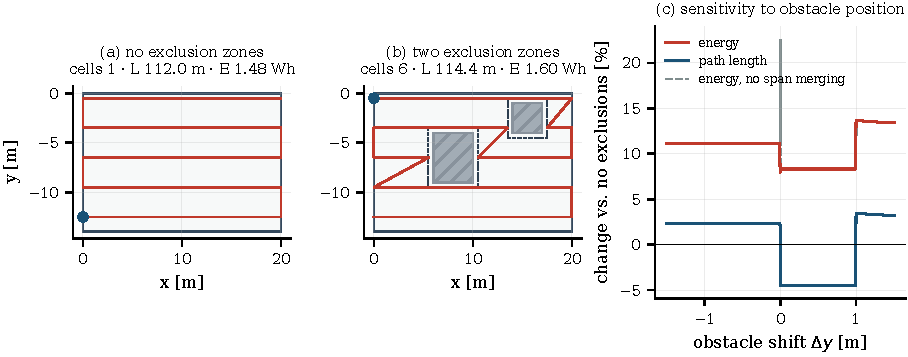
\includegraphics[width=\textwidth]{fig2_coverage.pdf}
  \caption{(a,b) Plans without and with the two exclusion zones (hatched; dashed:
  inflated by the $0.5$~m clearance); exact and greedy ordering give plans of
  equal length, time and energy here, flown in a different order. (c) Change in energy and path length caused by the exclusions when
  both obstacles are shifted by $\Delta y$; a planner without span merging (dashed grey)
  departs from ours only where scan rows lie on inflated obstacle
  edges ($\Delta y=0$ and $1$~m).}
  \label{fig:coverage}
\end{figure*}

On the reference field as placed (Table~\ref{tab:coverage},
Fig.~\ref{fig:coverage}a,b) the exclusions lengthen the plan by $\pubdL\%$ and raise its energy by
$\pubdE\%$; per accessible area, which shrinks by $\pubAreaLoss\%$, the increase
is $\pubdEarea\%$. Energy tracks mission time ($+\pubdT\%$) because, at this
speed, planning energy is hover power times time: each additional cell adds
rest-to-rest segments and transit that cost time but little length.

A planner that does not merge touching spans gives, for the same field,
$\subCells$ cells, $+\subdL\%$ length and $+\subdE\%$ energy. That value is a
degeneracy: with integer obstacle coordinates, a $0.5$~m clearance and rows at
$1.5$~m from the field edge and then every $3$~m, three rows lie exactly on inflated obstacle edges, and such a
planner splits each into touching spans that open spurious cells. Of the
$\subShiftN$ positions swept with it (dashed in
Fig.~\ref{fig:coverage}c), only the reference one produces it. Rows also meet inflated edges at $\Delta y=1$~m, and even with
span merging the reference position remains a special case: it is the
unique minimum of the sweep. Over the other $\genN$ positions the energy
increase spans $\gendEmin$--$\gendEmax\%$ (median $\gendEmed\%$) while the
length change spans $\gendLmin$ to $+\gendLmax\%$: in $\genShorter\%$ of the
positions the exclusions \emph{shorten} the plan and still cost more energy. The cost is a step function
of where the rows fall relative to the obstacles, so a single field cannot
characterize it.

Over the $\rndN$ random plans the per-scenario median increases are
$\rnddLmed\%$ in length (IQR $\rnddLlo$--$\rnddLhi\%$) and $\rnddEmed\%$ in
energy (IQR $\rnddElo$--$\rnddEhi\%$, 5th--95th percentile
$\rnddEfive$--$\rnddEninetyfive\%$). The median of the per-scenario ratio
$\Delta E/\Delta L$ is $\rndRatioMed$ (IQR $\rndRatioLo$--$\rndRatioHi$; over
the $\rndRatioN$ plans with $|\Delta L|>0.1\%$, $\rndRatioNeg$ of them negative),
and the ratio of the medians is $\rndRatioOfMedians$; the median ratio grows
with the number of exclusion zones ($\rndRatioKOne$, $\rndRatioKTwo$ and
$\rndRatioKThree$ for one, two and three); in $\rndShorter\%$ of
scenarios length falls while energy rises. Restricting to the $\rndCovN$ plans
with accessible coverage $\geq0.98$ with and without exclusions gives a median
energy increase of $\rndCovdEmed\%$. Pooled totals give $+\rndTotdL\%$ length and
$+\rndTotdE\%$ energy. No plan entered an inflated obstacle; none was refused, because
the generator keeps exclusions 1~m inside the field and 1.5~m apart.

\textbf{Cell ordering.} The $\subTransitCut\%$ transit reduction that exact
ordering shows on this field with the spurious cells also comes from them;
without them, exact and greedy ordering give
plans of \pubGreedyEqual\ length, time and energy, traversed in a different
order. Over the random plans greedy ordering costs a median
$\rndGreedyMed\%$ more energy than exact ordering ($>1\%$ in $\rndGreedyOne\%$ of
plans, $>5\%$ in $\rndGreedyFive\%$), and can be up to $\rndGreedyBest\%$
cheaper, since exact ordering minimizes transit length, not energy.

\subsection{Closed-loop execution}

\begin{figure*}[t]
  \centering
  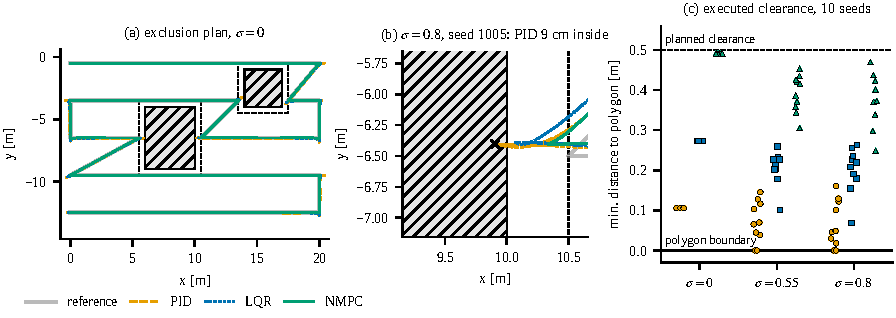
\includegraphics[width=\textwidth]{fig_clearance.pdf}
  \caption{Planned versus executed clearance on the exclusion plan (raw
  polygons hatched; dashed: inflated by the planned $0.5$~m). (a)~Reference
  and executed tracks without disturbance. (b)~The deepest of the saved
  $\sigma=0.8$ intrusions (exact order): PID overshoots a row end while braking
  and enters the polygon ($\times$).
  (c)~Minimum distance from each executed track to the raw polygons, 10 seeds
  per cell (at $\sigma=0$ the seeds coincide). Tracks are the episodes of
  Table~\ref{tab:clearance}, re-run with identical metrics.}
  \label{fig:clearance}
\end{figure*}

\begin{table}[t]
\caption{Closed loop on the exclusion plan (exact order): RMSE [m], minimum distance from the
executed track to the raw no-fly polygons [m] over 10 seeds, episodes below the
planned $0.5$~m clearance and episodes entering a no-fly polygon}
\label{tab:clearance}
\centering
\footnotesize
\setlength{\tabcolsep}{3.3pt}
\begin{tabular}{lcccccc}
\toprule
 & $\sigma$ & RMSE & min & median & $<0.5$~m & inside \\
\midrule
PID & 0.00 & 0.213 & 0.106 & 0.106 & 10/10 & 0/10 \\
PID & 0.55 & 0.245 & 0.000 & 0.068 & 10/10 & 2/10 \\
PID & 0.80 & 0.272 & 0.000 & 0.047 & 10/10 & 2/10 \\
LQR & 0.00 & 0.187 & 0.273 & 0.273 & 10/10 & 0/10 \\
LQR & 0.55 & 0.242 & 0.101 & 0.221 & 10/10 & 0/10 \\
LQR & 0.80 & 0.267 & 0.068 & 0.214 & 10/10 & 0/10 \\
NMPC & 0.00 & 0.013 & 0.491 & 0.491 & 10/10 & 0/10 \\
NMPC & 0.55 & 0.100 & 0.306 & 0.401 & 10/10 & 0/10 \\
NMPC & 0.80 & 0.122 & 0.249 & 0.371 & 10/10 & 0/10 \\
\bottomrule
\end{tabular}

\end{table}

Flying the exclusion plan preserves the planning ranking: without
disturbance executed energy exceeds planned energy by
$\execOverPlanLo$--$\execOverPlanHi\%$, and the exclusion premium measured in
closed loop, paired by seed against the same controller and wind on the free
field, is $\execdElo$--$\execdEhi\%$, against $\pubdE\%$ planned. With
$\sigma>0$ the persistent bias has a vertical component that shifts an
episode's energy by several percent either way, which is why only paired
comparisons are meaningful.

Planned clearance is not executed clearance (Table~\ref{tab:clearance},
Fig.~\ref{fig:clearance}). Rows
run along the inflated edges, so the reference itself sits at $0.5$~m, and every
controller drops below it in every episode, even without disturbance. The
NMPC keeps at least $\fairNmpcClr$~m;
LQR comes within $0.07$~m; PID enters a no-fly polygon in 2 of 10 episodes at
$\sigma=0.55$ and at $\sigma=0.8$, through overshoot when braking at row ends
that face an obstacle. Flown in the greedy order, the same plan gives PID
intrusions in 1 and 5 of 10 episodes and brings LQR within $0.05$~m: the executed
clearance may depend on the traversal order, which the planning metrics do not
see (2 against 5 of 10 PID intrusions at $\sigma=0.8$, Fisher $p=0.35$: not
resolved by 10 seeds). The PID--LQR difference is not statistically significant at this
sample size; with reference feedforward neither baseline enters a polygon in
the exact order (Sec.~V-C).

\subsection{Tracking: Monte Carlo against baselines}

\begin{table}[t]
\caption{Tracking RMSE [m], mean $\pm$ std over 30 seeds per cell}
\label{tab:mc}
\centering
\footnotesize
\setlength{\tabcolsep}{3pt}
\begin{tabular}{lcccc}
\toprule
$\sigma$ & \textbf{PID} & \textbf{LQR} & \textbf{NMPC} & \textbf{$\Delta$ vs best} \\
\midrule
0.00 & $0.181\pm0.000$ & $0.167\pm0.000$ & $\mathbf{0.013\pm0.000}$ & $-92.2\%$ \\
0.30 & $0.191\pm0.005$ & $0.209\pm0.010$ & $\mathbf{0.083\pm0.007}$ & $-56.7\%$ \\
0.55 & $0.212\pm0.009$ & $0.226\pm0.011$ & $\mathbf{0.101\pm0.007}$ & $-52.4\%$ \\
0.80 & $0.242\pm0.012$ & $0.251\pm0.013$ & $\mathbf{0.124\pm0.008}$ & $-48.8\%$ \\
\bottomrule
\end{tabular}
\end{table}

Table~\ref{tab:mc} reports the 360-mission campaign; a re-run with the
versioned scripts reproduces Table~\ref{tab:mc} to three decimals. The NMPC
reduces RMSE by $48.8$--$92.2\%$ relative to the better linear baseline at every
wind level, with no divergences. At $\sigma=0$ the 30 episodes per controller are
identical (no turbulence and no bias), so that row is a single run.

The energy differences between controllers are small but not null. Paired by
seed over the $\enPairs$ episodes with $\sigma>0$, the NMPC uses
$\enNP$~mWh ($\enNPrel\%$; 95\% CI $\enNPlo$ to $\enNPhi$) relative to PID
(paired $t$-test \enNPp) and $\enNL$~mWh ($\enNLrel\%$; CI $\enNLlo$ to
$\enNLhi$; \enNLp) relative to LQR, a difference whose sign changes with the wind
level and between the deposited run and the re-run. All differences lie within a $\pm1\%$
equivalence margin, so the energy effects of Table~\ref{tab:coverage} belong to
the plan, not to the controller tracking it.

\textbf{How much of the margin is the controller?} The NMPC sees the reference
over its whole horizon; the baselines see only the current position and
velocity reference. On the exclusion plan at $\sigma=0.55$, giving PID and LQR
the reference acceleration as feedforward lowers their RMSE from $\fairPid$ and
$\fairLqr$ to $\fairPidFf$ and $\fairLqrFf$~m, and removing the preview from the
NMPC (current reference extrapolated with its velocity, as in our ROS~2 node)
raises its RMSE from $\fairNmpc$ to $\fairNmpcEx$~m, between the two
feedforward baselines although it receives no reference acceleration. With feedforward no baseline enters a no-fly polygon in
30 episodes (PID without it: $\fairPidIn$). The preview thus accounts for
$\fairPreviewLo$--$\fairPreviewHi\%$ of the NMPC's margin over the original
baselines ($\sigma=0.55$, $0.8$); with feedforward, PID tracks better and LQR
worse than the NMPC without preview in all 20 paired episodes, so the
information is not matched exactly; without preview the NMPC also uses
$\fairNmpcExEnergy\%$ more energy.

NMPC solve times, measured on a desktop CPU during the 4-way parallel re-run,
average $\solveMeanLo$--$\solveMeanHi$~ms per episode (median 99th percentile
$\solvePnnMed$~ms) against the 10~ms budget, but the slowest solve exceeds it
in $\solveOverBudget$ of $\solveEpisodes$ episodes (up to $\solveMax$~ms); in the
original campaign of Table~\ref{tab:mc}, whose load conditions were not recorded (means
$\solveOrigMeanLo$--$\solveOrigMeanHi$~ms), it did so in all $\solveOrigOver$.
These are desktop figures under load, not embedded ones.

\subsection{Actuation delay}

\begin{figure}[t]
  \centering
  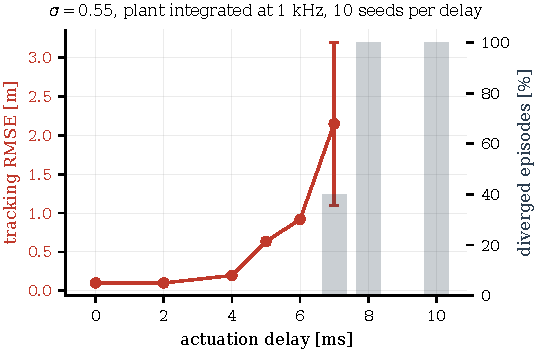
\includegraphics[width=\columnwidth]{fig4_delay.pdf}
  \caption{Uncompensated actuation delay at $\sigma=0.55$ (free field, plant at
  1~kHz, 10 seeds per delay): RMSE of runs below the 25~m criterion and share of diverged episodes.}
  \label{fig:delay}
\end{figure}

Up to 2~ms the delay is invisible beside the wind-driven error; RMSE roughly
doubles at 4~ms and is $9.2\times$ nominal at 6~ms. At 5--6~ms no episode
exceeds the 25~m divergence criterion, yet the vehicle inverts in all 10 episodes (3--35
inversions each; none at 4~ms): attitude control is lost between 4 and 5~ms. At 7~ms
\divSevenSub{} of 10 episodes diverged in one run and \divSevenRe{}
of 10 in a re-run with a newer solver build, which agree on only
\divSevenSame{} of the 10 seeds; from 8~ms all episodes diverge, accompanied by thousands of solver
failures. This is an empirical transition for this controller, fallback policy
and scenario --- not a stability margin --- and at 7~ms the divergence rate is
not resolved by 10 seeds.

\subsection{Perception}



NDVI separates healthy canopy ($0.851$) from diseased ($0.428$) and bare soil
($0.091$), NDWI $0.249$ from $-0.048$. Over 30 test trials at the calibrated
$\tau=0.65$, flagged zones reach precision $0.683\pm0.216$, recall
$0.641\pm0.247$ and $F_1=0.607\pm0.200$ (mean $\pm$ s.d.); $\tau$ lies
close to a steep drop of the calibration curve, so these values are sensitive to
it. The signatures and the ground truth share a generator, so this benchmark
measures the chain from indices to zones, not detection of real disease. A single Gazebo Classic
mission ($N=1$, threshold chosen on it; in the repository) only shows that
georeferencing closes end to end.

\section{Discussion and Limitations}
\label{sec:disc}

Without the degeneracy, for a rest-to-rest sweep path length understates the energy cost of exclusion zones by a factor that varies
with geometry (median $\rndRatioMed$ over random plans, with opposite signs in
some configurations). Planners that score time or energy~\cite{difranco2015energy,datsko2024energy,bahnemann2019gtsp}
already account for this; ours, which orders cells over two entry corners and
minimizes transit length, is not competitive with them. What this study adds is
the closed-loop side: the ranking survived execution, the planned clearance did not. Because planning energy here is hover power times
flight time, the ranking is in effect a time ranking: faster cruise or smooth
turns would change its magnitudes, which we did not evaluate.

The clearance a plan must reserve depends on the controller that flies it: in Table~\ref{tab:clearance} the
NMPC consumed up to half of the $0.5$~m margin under disturbance, LQR nearly all of it, and PID
all of it in some episodes, and plans of equal planned cost flown in different
orders may consume it differently. A controller-specific inflation, or a planner scoring predicted tracking
error at row ends, is the natural extension (not evaluated here). With control lost at 4--5~ms of delay and desktop means of
$\solveMeanLo$--$\solveOrigMeanHi$~ms (maxima above 10~ms), embedded deployment
needs a latency analysis we do not provide.

Results assume rest-to-rest segments (smooth
turns were not evaluated) and a world-frame force without airspeed coupling
(relative-airspeed turbulence is open). The NMPC has a
perfect model, and the ablation matches reference information only
approximately. The plan depends on the frame: rotating the field moves the
energy increase from 6.0 to 20.7\% over 72 angles, a $\pm1$~mm tolerance where
rows meet inflated edges moves it from 8.0 to 17.7\%, and rows can skip narrow
strips (free-field coverage $<0.98$ in 135 of 600 plans). All results are
simulated with zero computation delay on a non-identified airframe (thrust up
to $26\times$ weight), and both energies are model outputs (the planning model
omits acceleration thrust; the closed-loop one uses a different rotor model),
not measured battery consumption.

\section{Conclusion}

\emph{Observed.} For a rest-to-rest boustrophedon sweep, two exclusion zones
on a $20\times14$~m field change the plan length by $\gendLmin$ to
$+\gendLmax\%$ but cost $\gendEmin$--$\gendEmax\%$ more energy at generic
positions ($\pubdE\%$ at the reference one), because they
add stops and transits; a larger effect at the reference position, and a
benefit of exact cell ordering there, come from a degenerate decomposition.
\emph{Within this benchmark}, over $\rndN$ random plans the median costs are
$\rnddLmed\%$ in length and $\rnddEmed\%$ in energy, the planning ranking
survives closed-loop flight in the cases tested, part of the NMPC's tracking
advantage is reference preview, and no controller keeps the planned clearance,
which may also depend on the traversal order. \emph{Not shown}: energies measured on
a battery, a physically identified airframe, smooth-turn profiles, or
execution on embedded hardware. Planning that accounts for the tracking error
of the controller that will fly the plan is the natural next step.

\section*{Reproducibility}

The planner (with regression tests), plant, controller, Monte-Carlo harness,
input data with provenance records and the scripts that regenerate the numbers,
Tables I--II and the figures (\code{make\_numbers.py},
\code{coverage\_study.py}, \code{make\_figures.py}, \code{fig\_clearance.py})
are available at \url{https://github.com/JoseSegundoM/uav_energy_coverage}.
Input data carry SHA-256
checksums and every episode records its seed; \code{make\_numbers.py}
regenerates the numbers and Tables I--II byte for byte, and Table III matches
\code{mc\_main.json}.

\bibliographystyle{IEEEtran_doi}
\bibliography{refs}

\end{document}
.
% Requires \PaperTitle, \PaperAuthors (UTF-8, hyperref) and \PaperAuthorsPDF
% (PDFDocEncoding octal escapes, \pdfinfo) to be defined first.
\ifdefined\PDFPROFILE\else\def\PDFPROFILE{ieee}\fi
\def\profileinteractive{interactive}
\usepackage{tikz}
\usetikzlibrary{svg.path}
\definecolor{orcidlogocol}{HTML}{A6CE39}
% ORCID iD logo, same artwork as the orcidlink package (vector, no Type 3).
\newlength{\orcidxheight}
\newcommand{\orcidlogo}{\setlength{\orcidxheight}{\fontcharht\font`X}%
  \mbox{\begin{tikzpicture}[yscale=-0.00390625*\orcidxheight,
      xscale=0.00390625*\orcidxheight,transform shape]
    \fill[orcidlogocol] svg{M256,128c0,70.7-57.3,128-128,128C57.3,256,0,198.7,0,128C0,57.3,57.3,0,128,0C198.7,0,256,57.3,256,128z};
    \fill[white] svg{M86.3,186.2H70.9V79.1h15.4v48.4V186.2z}
      svg{M108.9,79.1h41.6c39.6,0,57,28.3,57,53.6c0,27.5-21.5,53.6-56.8,53.6h-41.8V79.1z M124.3,172.4h24.5c34.9,0,42.9-26.5,42.9-39.7c0-21.5-13.7-39.7-43.7-39.7h-23.7V172.4z}
      svg{M88.7,56.8c0,5.5-4.5,10.1-10.1,10.1c-5.6,0-10.1-4.6-10.1-10.1c0-5.6,4.5-10.1,10.1-10.1C84.2,46.7,88.7,51.3,88.7,56.8z};
  \end{tikzpicture}}}
\ifx\PDFPROFILE\profileinteractive
  \usepackage[colorlinks=true,linkcolor=black,citecolor=black,urlcolor=blue,
              bookmarks=false]{hyperref}
  \hypersetup{pdftitle={\PaperTitle},pdfauthor={\PaperAuthors}}
  \newcommand{\orcid}[1]{\href{https://orcid.org/#1}{\orcidlogo}}
  \newcommand{\authoremail}[1]{\href{mailto:#1}{#1}}
  \newcommand{\doititle}[2]{\href{https://doi.org/#1}{#2}}
  \newcommand{\urltitle}[2]{\href{#1}{#2}}
\else
  \pdfinfo{/Title (\PaperTitle) /Author (\PaperAuthorsPDF)}
  \newcommand{\orcid}[1]{\orcidlogo}
  \newcommand{\authoremail}[1]{#1}
  \newcommand{\doititle}[2]{#2}
  \newcommand{\urltitle}[2]{#2}
\fi

\usetikzlibrary{positioning,fit,backgrounds,calc,arrows.meta}
% Coauthor ORCID iDs (found in the BLADE_mars_coaxial CITATION.cff and on
% orcid.org) are shown only after each coauthor confirms them personally.
\newif\ifcoauthororcid \coauthororcidtrue
\newcommand{\coorcid}[1]{\ifcoauthororcid\,\orcid{#1}\fi}
% Affiliation confirmed by the corresponding author (2026-10-23) for all authors.
\newcommand{\paperaffiliation}{Universidad Nacional de Ingenier\'ia (UNI), Faculty of
  Mechanical Engineering, Lima, Peru}


\graphicspath{{figures/}}
\newcommand{\code}[1]{\texttt{\small #1}}
% Every number below comes from scripts/make_numbers.py (data/*.json).
% Generated by scripts/make_numbers.py -- do not edit by hand.
\newcommand{\divSevenRe}{6}
\newcommand{\divSevenSame}{4}
\newcommand{\divSevenSub}{4}
\newcommand{\edgeOnedE}{13.6}
\newcommand{\enNL}{-0.4}
\newcommand{\enNLhi}{0.1}
\newcommand{\enNLlo}{-0.9}
\newcommand{\enNLp}{$p=0.10$}
\newcommand{\enNLrel}{-0.03}
\newcommand{\enNP}{-10.2}
\newcommand{\enNPhi}{-9.9}
\newcommand{\enNPlo}{-10.5}
\newcommand{\enNPp}{$p<10^{-6}$}
\newcommand{\enNPrel}{-0.67}
\newcommand{\enPairs}{90}
\newcommand{\exclEpisodes}{90}
\newcommand{\execOverPlanHi}{1.8}
\newcommand{\execOverPlanLo}{1.0}
\newcommand{\execdEhi}{9.1}
\newcommand{\execdElo}{7.4}
\newcommand{\fairLqr}{0.242}
\newcommand{\fairLqrClr}{0.068}
\newcommand{\fairLqrFf}{0.188}
\newcommand{\fairLqrFfClr}{0.154}
\newcommand{\fairLqrFfIn}{0}
\newcommand{\fairLqrIn}{0}
\newcommand{\fairNmpc}{0.100}
\newcommand{\fairNmpcClr}{0.249}
\newcommand{\fairNmpcEx}{0.160}
\newcommand{\fairNmpcExClr}{0.134}
\newcommand{\fairNmpcExEnergy}{1.9}
\newcommand{\fairNmpcExIn}{0}
\newcommand{\fairNmpcIn}{0}
\newcommand{\fairPid}{0.245}
\newcommand{\fairPidClr}{0.000}
\newcommand{\fairPidFf}{0.145}
\newcommand{\fairPidFfClr}{0.216}
\newcommand{\fairPidFfIn}{0}
\newcommand{\fairPidIn}{4}
\newcommand{\fairPreviewHi}{42}
\newcommand{\fairPreviewLo}{35}
\newcommand{\genN}{299}
\newcommand{\genShorter}{33}
\newcommand{\gendEmax}{13.6}
\newcommand{\gendEmed}{11.1}
\newcommand{\gendEmin}{8.3}
\newcommand{\gendLmax}{3.4}
\newcommand{\gendLmin}{-4.5}
\newcommand{\pubAreaLoss}{16.4}
\newcommand{\pubCells}{6}
\newcommand{\pubGreedyEqual}{identical}
\newcommand{\pubdE}{8.0}
\newcommand{\pubdEarea}{29.2}
\newcommand{\pubdL}{2.2}
\newcommand{\pubdT}{8.0}
\newcommand{\rndCovN}{422}
\newcommand{\rndCovdEmed}{8.6}
\newcommand{\rndFields}{200}
\newcommand{\rndGreedyBest}{2.8}
\newcommand{\rndGreedyFive}{8}
\newcommand{\rndGreedyMed}{0.7}
\newcommand{\rndGreedyOne}{46}
\newcommand{\rndInvade}{0}
\newcommand{\rndN}{600}
\newcommand{\rndRatioHi}{3.47}
\newcommand{\rndRatioKOne}{1.77}
\newcommand{\rndRatioKThree}{3.02}
\newcommand{\rndRatioKTwo}{2.62}
\newcommand{\rndRatioLo}{1.54}
\newcommand{\rndRatioMed}{2.26}
\newcommand{\rndRatioN}{592}
\newcommand{\rndRatioNeg}{75}
\newcommand{\rndRatioOfMedians}{2.74}
\newcommand{\rndRefused}{0}
\newcommand{\rndShorter}{13}
\newcommand{\rndTotdE}{7.8}
\newcommand{\rndTotdL}{2.5}
\newcommand{\rnddEfive}{2.4}
\newcommand{\rnddEhi}{12.9}
\newcommand{\rnddElo}{5.6}
\newcommand{\rnddEmed}{8.8}
\newcommand{\rnddEninetyfive}{23.0}
\newcommand{\rnddLhi}{5.3}
\newcommand{\rnddLlo}{1.2}
\newcommand{\rnddLmed}{3.2}
\newcommand{\shiftGreedyMax}{0.4}
\newcommand{\shiftN}{301}
\newcommand{\shiftShareShorter}{33}
\newcommand{\shiftdEmax}{13.6}
\newcommand{\shiftdEmed}{11.1}
\newcommand{\shiftdEmin}{8.0}
\newcommand{\shiftdLmax}{3.4}
\newcommand{\shiftdLmin}{-4.5}
\newcommand{\solveEpisodes}{120}
\newcommand{\solveMax}{32.9}
\newcommand{\solveMeanHi}{2.76}
\newcommand{\solveMeanLo}{1.33}
\newcommand{\solveOrigMeanHi}{4.39}
\newcommand{\solveOrigMeanLo}{3.05}
\newcommand{\solveOrigOver}{120}
\newcommand{\solveOverBudget}{33}
\newcommand{\solvePnnMed}{2.91}
\newcommand{\subCells}{9}
\newcommand{\subShiftN}{305}
\newcommand{\subShiftSpikeN}{1}
\newcommand{\subTransitCut}{43}
\newcommand{\subdE}{22.6}
\newcommand{\subdEprinted}{22.7}
\newcommand{\subdL}{6.8}


\begin{document}

\title{Evaluating UAV Coverage Plans Beyond Path Length\\Using
Embedded-Deployable Nonlinear Model Predictive Control}

\author{\IEEEauthorblockN{Jose Luis Segundo Manayay\textsuperscript{*}\,\orcid{0009-0002-9203-8710},
Javier Yanpier Garay Yovera\coorcid{0009-0001-1645-8724},\\
Francisco Jes\'us Rodr\'iguez Huiman\coorcid{0009-0006-6972-2484},
Luis Angel Vilcamiche Fernandez\coorcid{0009-0005-7046-6943}}
\IEEEauthorblockA{\paperaffiliation\\
\authoremail{jose.segundo.m@uni.pe}; \authoremail{javier.garay.y@uni.pe};
\authoremail{francisco.rodriguez.h@uni.pe}; \authoremail{luis.vilcamiche.f@uni.pe}\\
{\footnotesize $^{*}$Corresponding author}}}

\maketitle

\begin{abstract}
Coverage path planners for agricultural UAVs are commonly ranked by path length.
We test, in closed-loop simulation, how well length predicts the energy a
multirotor spends on a boustrophedon plan flown with a rest-to-rest speed
profile. On a $20\times14$~m field, two exclusion zones change the plan length
by $\gendLmin$ to $+\gendLmax\%$ but raise its energy by
$\gendEmin$--$\gendEmax\%$ (median $\gendEmed\%$) over $\genN$ generic positions
($\pubdE\%$ at the reference one), because the
extra cells add stops and transits; planning energy is essentially hover power
times flight time. A larger value, $\subdE\%$, arises only from a
degenerate decomposition that occurs when scan rows lie exactly on inflated
obstacle edges. Over $\rndN$ random field, exclusion and sweep-direction
combinations the median increases are $\rnddLmed\%$ in length and
$\rnddEmed\%$ in energy. Flying the plans in closed loop, with a
C-code-generated NMPC (\code{acados}) and PID/LQR baselines under
Ornstein--Uhlenbeck force disturbances, preserves the planning-model ranking in
the cases tested. The NMPC reduces tracking RMSE by $49$--$92\%$ over the
baselines; an ablation attributes $\fairPreviewLo$--$\fairPreviewHi\%$ of that
margin to its reference preview; given the reference acceleration as
feedforward, PID tracks better and LQR worse than the NMPC without preview.
Every controller comes closer to the no-fly polygons than the planned
$0.5$~m clearance, even without disturbance, and executed clearance, which the
planning metrics do not show, can differ between traversal orders of equal
planned cost.
\end{abstract}

\begin{IEEEkeywords}
coverage path planning, model predictive control, energy-aware planning,
software-in-the-loop, precision agriculture, benchmarking
\end{IEEEkeywords}

\section{Introduction}

Coverage path planning for agricultural UAVs is a mature field, and its results
are often reported as path length, number of passes, or covered
area~\cite{galceran2013survey,hoffmann2024guidance}. These are properties of a
\emph{curve}. What a battery pays for is a \emph{trajectory}: a multirotor flying
a boustrophedon sweep with a rest-to-rest profile decelerates at every turn and
traverses whatever transit the cell structure imposes. That length is a poor
proxy for energy is known~\cite{datsko2024energy,bahnemann2019gtsp}; this paper
asks how the gap behaves for a stop-and-turn agricultural sweep with exclusion
zones, how much it depends on the geometry, and whether it survives
closed-loop execution. Answering it requires a planner, a plant, a controller, a disturbance model and
an energy model that are consistent with one another; we build that loop in
software. Our contributions are:

\begin{enumerate}
  \item \textbf{A closed-loop coverage benchmark} in which plans are scored both
        by a planning energy model and by the energy and clearance of the
        trajectory a controller actually flies.
  \item \textbf{A geometric sensitivity study of the length--energy gap} over
        obstacle positions and random fields, including a degenerate case that
        inflates the reference value.
  \item \textbf{An executed-safety measurement}: planned clearance is not
        executed clearance, even without disturbance.
  \item \textbf{A paired evaluation} of NMPC against PID and LQR baselines
        over 360 missions, with an ablation that separates control law from
        reference information, and a delay sweep.
\end{enumerate}
We claim no new control theory and no new planner: the predictive controller is
reused from prior work, and the planner is a standard boustrophedon
decomposition with Held--Karp cell ordering.

\section{Related Work}

\textbf{Coverage planning.} Galceran and Carreras~\cite{galceran2013survey}
survey the field; boustrophedon cellular
decomposition~\cite{choset1998boustrophedon} handles non-convex regions, and
Huang~\cite{huang2001optimal} shows that for convex polygons the sweep direction
minimizing passes is parallel to an edge. Agricultural guidance
tracks~\cite{hoffmann2024guidance} and wind-aware survey
decomposition~\cite{coombes2018polygon} extend this line. Bähnemann
\emph{et~al.}~\cite{bahnemann2019gtsp} pose cell ordering as a generalized TSP
with rest-to-rest time costs, and Datsko \emph{et~al.}~\cite{datsko2024energy}
plan multi-UAV coverage with an energy objective and optimal flight speed,
validated in flight. We do not propose a planner; we measure how a length
ranking and a planned clearance hold up against a closed-loop plant.

\textbf{Embedded predictive control.} CasADi~\cite{andersson2019casadi} and
\code{acados}~\cite{verschueren2022acados} with HPIPM~\cite{frison2020hpipm} and
real-time iteration~\cite{diehl2005rti} make nonlinear MPC tractable at 100~Hz.
We use this stack as a tool.

\textbf{Simulation and sensing.} Gazebo~\cite{koenig2004gazebo} with
ROS~2~\cite{macenski2022ros2} is the standard open stack. NDVI~\cite{rouse1974ndvi} and
NDWI~\cite{gao1996ndwi} are canonical vegetation indices; infected potato canopy
shows elevated visible and depressed NIR
reflectance~\cite{franceschini2019lateblight}; thermal CWSI
follows Idso~\emph{et al.}~\cite{idso1981cwsi}.

\section{Method}

\begin{figure*}[t]
  \centering
  % Fig. 1: evaluation architecture used for every closed-loop result
% (scripts/mc_experiments.py, Python). Solid: executed loop; dashed: exogenous
% inputs; dotted grey: auxiliary offline perception benchmark (no feedback).
\begin{tikzpicture}[x=1mm, y=1mm, font=\scriptsize, line width=0.55pt,
  >={Stealth[length=2.1mm, width=1.6mm]},
  blk/.style={draw, rounded corners=1.2pt, align=center, fill=white, inner sep=1.5pt},
  grp/.style={draw=black!35, rounded corners=3pt, line width=0.4pt},
  hdr/.style={font=\scriptsize\bfseries, anchor=south west, inner sep=0.8pt},
  flow/.style={->, line width=0.65pt}]
% ---------------- A. mission planning
\node[blk, minimum width=17mm, minimum height=10mm] (field) at (9,0) {field polygon\\+ exclusion\\zones};
\node[blk, minimum width=20mm, minimum height=10mm] (cells) at (31.5,0) {boustrophedon\\cells, routed\\row links};
\node[blk, minimum width=18mm, minimum height=10mm] (order) at (54,0) {cell ordering\\(Held--Karp)};
\node[blk, minimum width=20mm, minimum height=10mm] (ref) at (76.5,0) {timed reference\\rest-to-rest};
\draw[flow] (field) -- (cells); \draw[flow] (cells) -- (order); \draw[flow] (order) -- (ref);
% ---------------- B. flight control
\node[blk, minimum width=27mm, minimum height=9mm] (nmpc) at (113,8) {NMPC (\texttt{acados})\\$N{=}50$, $\Delta t{=}10$~ms};
\node[blk, minimum width=27mm, minimum height=9mm] (base) at (113,-8) {PID / LQR baselines\\(+FF in the ablation)};
\draw[flow] (ref.east) -- (91,0) |- (nmpc.west);
\node[anchor=east, inner sep=1pt] at (90.5,10) {$p_{\mathrm{ref}}$, 0.5~s ahead};
\draw[flow] (ref.east) -- (91,0) |- (base.west);
\node[anchor=east, inner sep=1pt] at (90.5,-10) {$p_{\mathrm{ref}}(t)$, $v_{\mathrm{ref}}(t)$};
% ---------------- delay and C. plant
\node[blk, minimum width=13mm, minimum height=9mm, fill=black!5] (delay) at (141,0) {delay\\buffer $\tau_d$};
\draw[flow] (nmpc.east) -- (132,8) |- (delay.west);
\draw[flow] (base.east) -- (132,-8) |- (delay.west);
\node at (130.2,2.4) {$\delta$};
\node[blk, minimum width=21mm, minimum height=13mm, fill=black!5] (plant) at (161,0) {18-state model:\\rotor speeds,\\quaternion; RK4,\\100~Hz / 1~kHz};
\draw[flow] (delay) -- (plant);
\draw[flow, densely dashed] (160,16.5) -- (160,8.6);
\node[anchor=east, inner sep=1pt] at (159.5,15.5) {OU force $f_w$};
% true-state feedback, one arrow per controller
\draw[flow] (169,8.6) -- (169,20) -- node[above, pos=0.5] {true state $x$ (no estimator)} (124,20) -- (124,12.5);
\draw[flow] (155,-8.6) -- (155,-16) -- node[below, pos=0.5] {true state $x$} (113,-16) -- (base.south);
% ---------------- D. evaluation
\node[blk, minimum width=108mm, minimum height=8mm] (eval) at (120,-28)
  {tracking RMSE $\cdot$ executed and planned energy $\cdot$ clearance to raw polygons $\cdot$ coverage\\solve time $\cdot$ divergence and inversions};
\draw[flow] (70,-5) -- (70,-23.9);
\draw[flow] (166,-8.6) -- (166,-23.9);
% ---------------- E. auxiliary perception (offline, no feedback)
\node[blk, draw=black!45, text=black!60, densely dotted, minimum width=46mm, minimum height=8mm] (perc) at (24,-28)
  {five-band synthetic mosaic $\to$ NDVI/NDWI\\$\to$ health index $\to$ flagged zones};
% ---------------- group frames and headers
\begin{scope}[on background layer]
\draw[grp, fill=blue!4] (-1,-7) rectangle (88,7);
\draw[grp, fill=orange!6] (97,-14) rectangle (129,14);
\draw[grp, fill=green!5] (148.5,-11) rectangle (173.5,11);
\end{scope}
\node[hdr] at (-1,7) {A\, mission planning};
\node[hdr] at (97,14) {B\, flight control};
\node[hdr] at (148.5,11) {C\, plant};
\node[hdr] at (73,-23.5) {D\, evaluation};
\node[hdr, text=black!55] at (1,-23.5) {E\, synthetic perception (auxiliary, offline)};
\end{tikzpicture}

  \caption{Evaluation architecture used for every closed-loop result, run in
  Python (no Gazebo or ROS~2 in the loop). (A)~The planner turns the field and
  exclusion zones into a timed rest-to-rest reference. (B)~The NMPC receives
  the reference over its 0.5~s horizon; PID and LQR receive the current
  position and velocity reference (plus the reference acceleration in the
  feedforward ablation). Both act on the true state. (C)~Rotor commands
  $\delta$ pass through an optional delay buffer (delay sweep) to the 18-state
  plant, integrated with RK4 at 100~Hz or 1~kHz under a world-frame
  Ornstein--Uhlenbeck force. (D)~Metrics. (E)~The synthetic perception
  benchmark is separate and offline.}
  \label{fig:arch}
\end{figure*}

\subsection{Vehicle model and disturbance}

The plant is the 18-state model
$x = [\,p^\top, v^\top, q^\top, \omega_b^\top, \varpi^\top, V_b\,]^\top$
with position $p$, world-frame (ENU) velocity $v$, attitude quaternion $q$, body
rates $\omega_b$, four rotor speeds $\varpi$ and battery voltage $V_b$. Rotor
$i$ produces thrust $k_f\varpi_i^2$ and reactive torque $k_m\varpi_i^2$; the
translational dynamics are
\begin{equation}
  m\dot v = R(q)\,\textstyle\sum_i k_f \varpi_i^2 \,e_3 - m g e_3
            - c_d \lVert v \rVert v + f_w ,
  \label{eq:trans}
\end{equation}
with $m=0.80$~kg, $k_f=2.3\times10^{-5}$~N$\cdot$s$^2$,
$k_m=7.0\times10^{-7}$~N$\cdot$m$\cdot$s$^2$ and $c_d=0.15$~kg/m. Rotor speeds
follow first-order actuator dynamics driven by normalized commands
$\delta\in[0,1]^4$; $V_b$ discharges with consumed current.

The disturbance $f_w$ is a \emph{world-frame} external force, not an airspeed:
an Ornstein--Uhlenbeck process
$\mathrm{d}f_w = -\theta f_w\,\mathrm{d}t + \sigma\,\mathrm{d}W$ with
$\theta=1$~s$^{-1}$ (stationary standard deviation $\sigma/\sqrt{2\theta}$ per
axis), plus, for $\sigma>0$ only, a constant per-episode bias of $0.6$~N whose
direction is drawn per seed. The drag in~(\ref{eq:trans}) uses ground velocity,
so the model has no relative-airspeed coupling. We keep it because the
controller was tuned against it; Section~\ref{sec:disc} states what this costs.

\subsection{Coverage planning}

The field is expressed in a local ENU frame; the sweep direction minimizes the
perpendicular extent of the hull~\cite{huang2001optimal}, and exclusion zones are
inflated by a $0.5$~m clearance and subtracted from the free area. Scan rows
intersect the free area in spans; spans on consecutive rows that overlap belong
to one cell, and a change in span count marks a critical point where cells close
and open~\cite{choset1998boustrophedon}. Three details matter for correctness:
(i) when a row lies exactly on an inflated obstacle edge, the free area (a
closed set) meets it in collinear spans that \emph{touch}; they are merged into
one span, since otherwise they read as critical points, create spurious cells
and force stops mid-row;
(ii) the link from one row to the next inside a cell, not only the transit
between cells, is routed around the inflated obstacles (on a visibility graph,
by Dijkstra);
(iii) if the free area is disconnected, the plan is refused rather than joined
by a segment through a no-fly zone. Each is covered by a regression test.

\textbf{Cell ordering} is an open-path TSP over cells and two traversal
directions with \emph{routed} transit lengths as edge costs, solved exactly by
Held--Karp over two of the four entry corners per cell; it minimizes transit
length, not energy or time. The planner emits a timed
reference $t\mapsto(x,y,z,\psi)$ with a trapezoidal speed profile (2~m/s cruise)
applied \emph{per segment}, so the vehicle comes to rest at every segment end.

\subsection{NMPC and baselines}

The OCP is formulated in CasADi and exported to C by \code{acados}: $N=50$
shooting nodes at $\Delta t=10$~ms, Gauss--Newton Hessians, explicit Runge--Kutta
integration, real-time iteration and partially condensed HPIPM. The attitude
term is $\lVert \mathrm{vec}(q_\mathrm{ref}^{*}\otimes q)\rVert^2=\sin^2(\alpha/2)$
for a relative rotation $\alpha$: invariant to the quaternion sign, but not the
squared geodesic distance. In the Monte-Carlo campaigns the NMPC receives the
reference over its whole horizon with a fixed yaw, while the PID and LQR
baselines, reused unchanged from the same prior work, act on the current
reference only; the
ROS~2 node instead extrapolates the reference and uses a measured-yaw governor.
The comparison is therefore not information-equivalent. We write
\emph{embedded-deployable} because the artefact is the generated C code; no
embedded processor executes it here, and we make no on-target timing claim.

\subsection{Energy model}

The planning model uses momentum theory with induced, profile and parasite
power,
\begin{equation}
  P_\mathrm{mech}(V) = k_i T v_i(V) + P_{p0}\!\left(1 + 4.65\mu^2\right)
                       + c_d V^3 ,
  \label{eq:power}
\end{equation}
with $v_i = v_h^2/\sqrt{V^2+v_i^2}$, advance ratio $\mu=V/(\Omega R)$ and the
same $c_d$ as~(\ref{eq:trans}); the effective disc area is calibrated so
that~(\ref{eq:power}) reproduces the plant's hover power ($82.0$~W electrical).
At 2~m/s it gives $82.2$~W, so planning energy is, within $0.2\%$, hover power
times mission time. For closed-loop runs we integrate
$P=\sum_i k_m\varpi_i^3/\eta$ from the simulated rotor speeds.

\subsection{Synthetic multispectral layer}

A procedurally generated five-band reflectance mosaic ($0.05$~m) with canopy,
soil and late-blight signatures~\cite{franceschini2019lateblight} feeds
NDVI~\cite{rouse1974ndvi} and NDWI~\cite{gao1996ndwi}, fused into a health index
$H=0.65\widehat{\mathrm{NDVI}}+0.35\widehat{\mathrm{NDWI}}$ that is thresholded
at $\tau$. Each trial randomizes foci, rows, illumination, noise and severity,
and $\tau$ is calibrated on trials disjoint from the test set.

\section{Experimental Design}

All missions cover a $20\times14$~m plot at 7~m AGL, 2~m/s and 3~m track
spacing, unless stated otherwise.
\textbf{Geometric sensitivity.} With the planning model only: the reference field
with both obstacles shifted rigidly in $y$ over $\pm1.5$~m in 1~cm steps
($\shiftN$ positions); and $\rndFields$ random rectangular fields
($15$--$60$~m, aspect $1$--$3$) with 1--3 exclusions (half of them rotated),
each planned along three sweep directions ($\rndN$ plans). Every relative change
is computed per scenario against the same field without exclusions.
\textbf{Monte Carlo.} PID, LQR and NMPC $\times$ $\sigma\in\{0,0.3,0.55,0.8\}$
N$\cdot$s$^{-1/2}$ $\times$ 30 seeds $=360$ episodes on the exclusion-free field,
plant at 100~Hz; seeds fix the OU realization and the bias direction.
\textbf{Closed loop with exclusions.} The three controllers on the
exclusion plan, $\sigma\in\{0,0.55,0.8\}$, 10 seeds ($\exclEpisodes$ episodes),
recording planned and executed energy and the minimum distance from the executed
track to the raw no-fly polygons.
\textbf{Delay sweep.} NMPC at $\sigma=0.55$ with uncompensated actuation delay
$\tau_d\in\{0,2,4,5,6,7,8,10\}$~ms, 10 seeds each, plant at 1~kHz; an episode
diverges if the state leaves a finite range or the position error exceeds 25~m.
\textbf{Perception.} 10 calibration trials to select $\tau$, then 30 disjoint
test trials.

\section{Results}

\subsection{Geometric cost understates dynamic cost --- by a geometry-dependent amount}

\begin{table}[t]
\caption{Coverage cost, $20\times14$~m plot, 3~m spacing (planning model)}
\label{tab:coverage}
\centering
\footnotesize
\setlength{\tabcolsep}{4pt}
\begin{tabular}{lccc}
\toprule
& \textbf{No exclusions} & \textbf{Exclusions} & \textbf{Exclusions} \\
& & \textbf{(exact)} & \textbf{(greedy)} \\
\midrule
Cells & 1 & 6 & 6 \\
Path length [m] & 112.0 & 114.4 & 114.4 \\
\quad transit [m] & --- & 20.4 & 20.4 \\
Mission time [s] & 65.0 & 70.2 & 70.2 \\
Free area [m$^2$] & 280.0 & 234.0 & 234.0 \\
Energy [Wh] & 1.483 & 1.602 & 1.602 \\
Energy/area [mWh\,m$^{-2}$] & 5.30 & 6.84 & 6.84 \\
Field coverage [\%] & 100.0 & 95.5 & 95.5 \\
Accessible coverage [\%] & 100.0 & 99.5 & 99.5 \\
\bottomrule
\end{tabular}

\end{table}

\begin{figure*}[t]
  \centering
  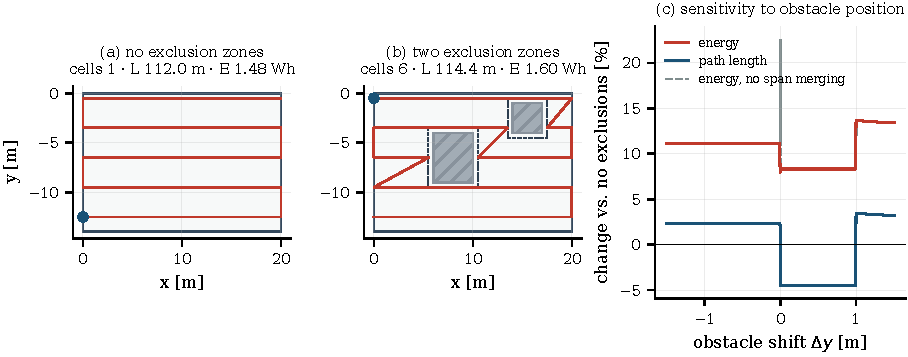
\includegraphics[width=\textwidth]{fig2_coverage.pdf}
  \caption{(a,b) Plans without and with the two exclusion zones (hatched; dashed:
  inflated by the $0.5$~m clearance); exact and greedy ordering give plans of
  equal length, time and energy here, flown in a different order. (c) Change in energy and path length caused by the exclusions when
  both obstacles are shifted by $\Delta y$; a planner without span merging (dashed grey)
  departs from ours only where scan rows lie on inflated obstacle
  edges ($\Delta y=0$ and $1$~m).}
  \label{fig:coverage}
\end{figure*}

On the reference field as placed (Table~\ref{tab:coverage},
Fig.~\ref{fig:coverage}a,b) the exclusions lengthen the plan by $\pubdL\%$ and raise its energy by
$\pubdE\%$; per accessible area, which shrinks by $\pubAreaLoss\%$, the increase
is $\pubdEarea\%$. Energy tracks mission time ($+\pubdT\%$) because, at this
speed, planning energy is hover power times time: each additional cell adds
rest-to-rest segments and transit that cost time but little length.

A planner that does not merge touching spans gives, for the same field,
$\subCells$ cells, $+\subdL\%$ length and $+\subdE\%$ energy. That value is a
degeneracy: with integer obstacle coordinates, a $0.5$~m clearance and rows at
$1.5$~m from the field edge and then every $3$~m, three rows lie exactly on inflated obstacle edges, and such a
planner splits each into touching spans that open spurious cells. Of the
$\subShiftN$ positions swept with it (dashed in
Fig.~\ref{fig:coverage}c), only the reference one produces it. Rows also meet inflated edges at $\Delta y=1$~m, and even with
span merging the reference position remains a special case: it is the
unique minimum of the sweep. Over the other $\genN$ positions the energy
increase spans $\gendEmin$--$\gendEmax\%$ (median $\gendEmed\%$) while the
length change spans $\gendLmin$ to $+\gendLmax\%$: in $\genShorter\%$ of the
positions the exclusions \emph{shorten} the plan and still cost more energy. The cost is a step function
of where the rows fall relative to the obstacles, so a single field cannot
characterize it.

Over the $\rndN$ random plans the per-scenario median increases are
$\rnddLmed\%$ in length (IQR $\rnddLlo$--$\rnddLhi\%$) and $\rnddEmed\%$ in
energy (IQR $\rnddElo$--$\rnddEhi\%$, 5th--95th percentile
$\rnddEfive$--$\rnddEninetyfive\%$). The median of the per-scenario ratio
$\Delta E/\Delta L$ is $\rndRatioMed$ (IQR $\rndRatioLo$--$\rndRatioHi$; over
the $\rndRatioN$ plans with $|\Delta L|>0.1\%$, $\rndRatioNeg$ of them negative),
and the ratio of the medians is $\rndRatioOfMedians$; the median ratio grows
with the number of exclusion zones ($\rndRatioKOne$, $\rndRatioKTwo$ and
$\rndRatioKThree$ for one, two and three); in $\rndShorter\%$ of
scenarios length falls while energy rises. Restricting to the $\rndCovN$ plans
with accessible coverage $\geq0.98$ with and without exclusions gives a median
energy increase of $\rndCovdEmed\%$. Pooled totals give $+\rndTotdL\%$ length and
$+\rndTotdE\%$ energy. No plan entered an inflated obstacle; none was refused, because
the generator keeps exclusions 1~m inside the field and 1.5~m apart.

\textbf{Cell ordering.} The $\subTransitCut\%$ transit reduction that exact
ordering shows on this field with the spurious cells also comes from them;
without them, exact and greedy ordering give
plans of \pubGreedyEqual\ length, time and energy, traversed in a different
order. Over the random plans greedy ordering costs a median
$\rndGreedyMed\%$ more energy than exact ordering ($>1\%$ in $\rndGreedyOne\%$ of
plans, $>5\%$ in $\rndGreedyFive\%$), and can be up to $\rndGreedyBest\%$
cheaper, since exact ordering minimizes transit length, not energy.

\subsection{Closed-loop execution}

\begin{figure*}[t]
  \centering
  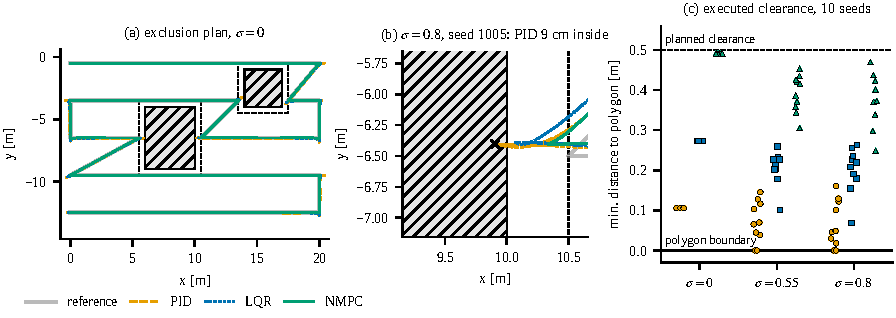
\includegraphics[width=\textwidth]{fig_clearance.pdf}
  \caption{Planned versus executed clearance on the exclusion plan (raw
  polygons hatched; dashed: inflated by the planned $0.5$~m). (a)~Reference
  and executed tracks without disturbance. (b)~The deepest of the saved
  $\sigma=0.8$ intrusions (exact order): PID overshoots a row end while braking
  and enters the polygon ($\times$).
  (c)~Minimum distance from each executed track to the raw polygons, 10 seeds
  per cell (at $\sigma=0$ the seeds coincide). Tracks are the episodes of
  Table~\ref{tab:clearance}, re-run with identical metrics.}
  \label{fig:clearance}
\end{figure*}

\begin{table}[t]
\caption{Closed loop on the exclusion plan (exact order): RMSE [m], minimum distance from the
executed track to the raw no-fly polygons [m] over 10 seeds, episodes below the
planned $0.5$~m clearance and episodes entering a no-fly polygon}
\label{tab:clearance}
\centering
\footnotesize
\setlength{\tabcolsep}{3.3pt}
\begin{tabular}{lcccccc}
\toprule
 & $\sigma$ & RMSE & min & median & $<0.5$~m & inside \\
\midrule
PID & 0.00 & 0.213 & 0.106 & 0.106 & 10/10 & 0/10 \\
PID & 0.55 & 0.245 & 0.000 & 0.068 & 10/10 & 2/10 \\
PID & 0.80 & 0.272 & 0.000 & 0.047 & 10/10 & 2/10 \\
LQR & 0.00 & 0.187 & 0.273 & 0.273 & 10/10 & 0/10 \\
LQR & 0.55 & 0.242 & 0.101 & 0.221 & 10/10 & 0/10 \\
LQR & 0.80 & 0.267 & 0.068 & 0.214 & 10/10 & 0/10 \\
NMPC & 0.00 & 0.013 & 0.491 & 0.491 & 10/10 & 0/10 \\
NMPC & 0.55 & 0.100 & 0.306 & 0.401 & 10/10 & 0/10 \\
NMPC & 0.80 & 0.122 & 0.249 & 0.371 & 10/10 & 0/10 \\
\bottomrule
\end{tabular}

\end{table}

Flying the exclusion plan preserves the planning ranking: without
disturbance executed energy exceeds planned energy by
$\execOverPlanLo$--$\execOverPlanHi\%$, and the exclusion premium measured in
closed loop, paired by seed against the same controller and wind on the free
field, is $\execdElo$--$\execdEhi\%$, against $\pubdE\%$ planned. With
$\sigma>0$ the persistent bias has a vertical component that shifts an
episode's energy by several percent either way, which is why only paired
comparisons are meaningful.

Planned clearance is not executed clearance (Table~\ref{tab:clearance},
Fig.~\ref{fig:clearance}). Rows
run along the inflated edges, so the reference itself sits at $0.5$~m, and every
controller drops below it in every episode, even without disturbance. The
NMPC keeps at least $\fairNmpcClr$~m;
LQR comes within $0.07$~m; PID enters a no-fly polygon in 2 of 10 episodes at
$\sigma=0.55$ and at $\sigma=0.8$, through overshoot when braking at row ends
that face an obstacle. Flown in the greedy order, the same plan gives PID
intrusions in 1 and 5 of 10 episodes and brings LQR within $0.05$~m: the executed
clearance may depend on the traversal order, which the planning metrics do not
see (2 against 5 of 10 PID intrusions at $\sigma=0.8$, Fisher $p=0.35$: not
resolved by 10 seeds). The PID--LQR difference is not statistically significant at this
sample size; with reference feedforward neither baseline enters a polygon in
the exact order (Sec.~V-C).

\subsection{Tracking: Monte Carlo against baselines}

\begin{table}[t]
\caption{Tracking RMSE [m], mean $\pm$ std over 30 seeds per cell}
\label{tab:mc}
\centering
\footnotesize
\setlength{\tabcolsep}{3pt}
\begin{tabular}{lcccc}
\toprule
$\sigma$ & \textbf{PID} & \textbf{LQR} & \textbf{NMPC} & \textbf{$\Delta$ vs best} \\
\midrule
0.00 & $0.181\pm0.000$ & $0.167\pm0.000$ & $\mathbf{0.013\pm0.000}$ & $-92.2\%$ \\
0.30 & $0.191\pm0.005$ & $0.209\pm0.010$ & $\mathbf{0.083\pm0.007}$ & $-56.7\%$ \\
0.55 & $0.212\pm0.009$ & $0.226\pm0.011$ & $\mathbf{0.101\pm0.007}$ & $-52.4\%$ \\
0.80 & $0.242\pm0.012$ & $0.251\pm0.013$ & $\mathbf{0.124\pm0.008}$ & $-48.8\%$ \\
\bottomrule
\end{tabular}
\end{table}

Table~\ref{tab:mc} reports the 360-mission campaign; a re-run with the
versioned scripts reproduces Table~\ref{tab:mc} to three decimals. The NMPC
reduces RMSE by $48.8$--$92.2\%$ relative to the better linear baseline at every
wind level, with no divergences. At $\sigma=0$ the 30 episodes per controller are
identical (no turbulence and no bias), so that row is a single run.

The energy differences between controllers are small but not null. Paired by
seed over the $\enPairs$ episodes with $\sigma>0$, the NMPC uses
$\enNP$~mWh ($\enNPrel\%$; 95\% CI $\enNPlo$ to $\enNPhi$) relative to PID
(paired $t$-test \enNPp) and $\enNL$~mWh ($\enNLrel\%$; CI $\enNLlo$ to
$\enNLhi$; \enNLp) relative to LQR, a difference whose sign changes with the wind
level and between the deposited run and the re-run. All differences lie within a $\pm1\%$
equivalence margin, so the energy effects of Table~\ref{tab:coverage} belong to
the plan, not to the controller tracking it.

\textbf{How much of the margin is the controller?} The NMPC sees the reference
over its whole horizon; the baselines see only the current position and
velocity reference. On the exclusion plan at $\sigma=0.55$, giving PID and LQR
the reference acceleration as feedforward lowers their RMSE from $\fairPid$ and
$\fairLqr$ to $\fairPidFf$ and $\fairLqrFf$~m, and removing the preview from the
NMPC (current reference extrapolated with its velocity, as in our ROS~2 node)
raises its RMSE from $\fairNmpc$ to $\fairNmpcEx$~m, between the two
feedforward baselines although it receives no reference acceleration. With feedforward no baseline enters a no-fly polygon in
30 episodes (PID without it: $\fairPidIn$). The preview thus accounts for
$\fairPreviewLo$--$\fairPreviewHi\%$ of the NMPC's margin over the original
baselines ($\sigma=0.55$, $0.8$); with feedforward, PID tracks better and LQR
worse than the NMPC without preview in all 20 paired episodes, so the
information is not matched exactly; without preview the NMPC also uses
$\fairNmpcExEnergy\%$ more energy.

NMPC solve times, measured on a desktop CPU during the 4-way parallel re-run,
average $\solveMeanLo$--$\solveMeanHi$~ms per episode (median 99th percentile
$\solvePnnMed$~ms) against the 10~ms budget, but the slowest solve exceeds it
in $\solveOverBudget$ of $\solveEpisodes$ episodes (up to $\solveMax$~ms); in the
original campaign of Table~\ref{tab:mc}, whose load conditions were not recorded (means
$\solveOrigMeanLo$--$\solveOrigMeanHi$~ms), it did so in all $\solveOrigOver$.
These are desktop figures under load, not embedded ones.

\subsection{Actuation delay}

\begin{figure}[t]
  \centering
  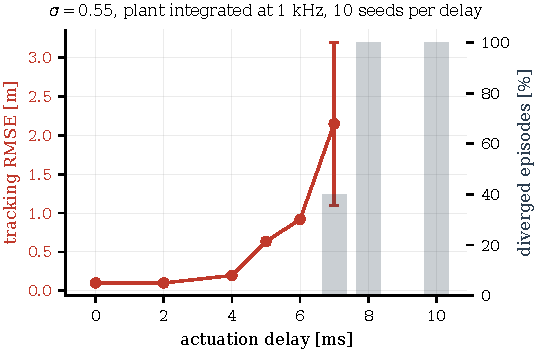
\includegraphics[width=\columnwidth]{fig4_delay.pdf}
  \caption{Uncompensated actuation delay at $\sigma=0.55$ (free field, plant at
  1~kHz, 10 seeds per delay): RMSE of runs below the 25~m criterion and share of diverged episodes.}
  \label{fig:delay}
\end{figure}

Up to 2~ms the delay is invisible beside the wind-driven error; RMSE roughly
doubles at 4~ms and is $9.2\times$ nominal at 6~ms. At 5--6~ms no episode
exceeds the 25~m divergence criterion, yet the vehicle inverts in all 10 episodes (3--35
inversions each; none at 4~ms): attitude control is lost between 4 and 5~ms. At 7~ms
\divSevenSub{} of 10 episodes diverged in one run and \divSevenRe{}
of 10 in a re-run with a newer solver build, which agree on only
\divSevenSame{} of the 10 seeds; from 8~ms all episodes diverge, accompanied by thousands of solver
failures. This is an empirical transition for this controller, fallback policy
and scenario --- not a stability margin --- and at 7~ms the divergence rate is
not resolved by 10 seeds.

\subsection{Perception}



NDVI separates healthy canopy ($0.851$) from diseased ($0.428$) and bare soil
($0.091$), NDWI $0.249$ from $-0.048$. Over 30 test trials at the calibrated
$\tau=0.65$, flagged zones reach precision $0.683\pm0.216$, recall
$0.641\pm0.247$ and $F_1=0.607\pm0.200$ (mean $\pm$ s.d.); $\tau$ lies
close to a steep drop of the calibration curve, so these values are sensitive to
it. The signatures and the ground truth share a generator, so this benchmark
measures the chain from indices to zones, not detection of real disease. A single Gazebo Classic
mission ($N=1$, threshold chosen on it; in the repository) only shows that
georeferencing closes end to end.

\section{Discussion and Limitations}
\label{sec:disc}

Without the degeneracy, for a rest-to-rest sweep path length understates the energy cost of exclusion zones by a factor that varies
with geometry (median $\rndRatioMed$ over random plans, with opposite signs in
some configurations). Planners that score time or energy~\cite{difranco2015energy,datsko2024energy,bahnemann2019gtsp}
already account for this; ours, which orders cells over two entry corners and
minimizes transit length, is not competitive with them. What this study adds is
the closed-loop side: the ranking survived execution, the planned clearance did not. Because planning energy here is hover power times
flight time, the ranking is in effect a time ranking: faster cruise or smooth
turns would change its magnitudes, which we did not evaluate.

The clearance a plan must reserve depends on the controller that flies it: in Table~\ref{tab:clearance} the
NMPC consumed up to half of the $0.5$~m margin under disturbance, LQR nearly all of it, and PID
all of it in some episodes, and plans of equal planned cost flown in different
orders may consume it differently. A controller-specific inflation, or a planner scoring predicted tracking
error at row ends, is the natural extension (not evaluated here). With control lost at 4--5~ms of delay and desktop means of
$\solveMeanLo$--$\solveOrigMeanHi$~ms (maxima above 10~ms), embedded deployment
needs a latency analysis we do not provide.

Results assume rest-to-rest segments (smooth
turns were not evaluated) and a world-frame force without airspeed coupling
(relative-airspeed turbulence is open). The NMPC has a
perfect model, and the ablation matches reference information only
approximately. The plan depends on the frame: rotating the field moves the
energy increase from 6.0 to 20.7\% over 72 angles, a $\pm1$~mm tolerance where
rows meet inflated edges moves it from 8.0 to 17.7\%, and rows can skip narrow
strips (free-field coverage $<0.98$ in 135 of 600 plans). All results are
simulated with zero computation delay on a non-identified airframe (thrust up
to $26\times$ weight), and both energies are model outputs (the planning model
omits acceleration thrust; the closed-loop one uses a different rotor model),
not measured battery consumption.

\section{Conclusion}

\emph{Observed.} For a rest-to-rest boustrophedon sweep, two exclusion zones
on a $20\times14$~m field change the plan length by $\gendLmin$ to
$+\gendLmax\%$ but cost $\gendEmin$--$\gendEmax\%$ more energy at generic
positions ($\pubdE\%$ at the reference one), because they
add stops and transits; a larger effect at the reference position, and a
benefit of exact cell ordering there, come from a degenerate decomposition.
\emph{Within this benchmark}, over $\rndN$ random plans the median costs are
$\rnddLmed\%$ in length and $\rnddEmed\%$ in energy, the planning ranking
survives closed-loop flight in the cases tested, part of the NMPC's tracking
advantage is reference preview, and no controller keeps the planned clearance,
which may also depend on the traversal order. \emph{Not shown}: energies measured on
a battery, a physically identified airframe, smooth-turn profiles, or
execution on embedded hardware. Planning that accounts for the tracking error
of the controller that will fly the plan is the natural next step.

\section*{Reproducibility}

The planner (with regression tests), plant, controller, Monte-Carlo harness,
input data with provenance records and the scripts that regenerate the numbers,
Tables I--II and the figures (\code{make\_numbers.py},
\code{coverage\_study.py}, \code{make\_figures.py}, \code{fig\_clearance.py})
are available at \url{https://github.com/JoseSegundoM/uav_energy_coverage}.
Input data carry SHA-256
checksums and every episode records its seed; \code{make\_numbers.py}
regenerates the numbers and Tables I--II byte for byte, and Table III matches
\code{mc\_main.json}.

\bibliographystyle{IEEEtran_doi}
\bibliography{refs}

\end{document}
